\documentclass[review]{elsarticle}
\usepackage{lineno,hyperref}
\usepackage{subcaption}
\usepackage{siunitx}
\sisetup{group-separator = {,}}
\usepackage{booktabs}
\usepackage{graphicx}
\usepackage{adjustbox}
\usepackage{appendix}
\usepackage{amsmath} 
\usepackage{scrextend}
\usepackage[hang,flushmargin]{footmisc} 
\usepackage{xcolor}
\usepackage{float}
\usepackage{array,multirow}
\usepackage{hyperref}
\usepackage{setspace}
\usepackage{stmaryrd}
\usepackage{enumitem}
\usepackage{rotating}
\usepackage{adjustbox}
\usepackage{array}
\usepackage{booktabs}
\usepackage{xcolor,colortbl}
\usepackage{amsmath} 
\usepackage{amsfonts} 
\usepackage{amssymb}
\usepackage{makecell}
\usepackage{amsmath}
\usepackage{nicefrac}
\usepackage{todonotes}
\usepackage{multirow}
\modulolinenumbers[1]
\usepackage{lineno}
\usepackage{tikz}
\usepackage{cleveref}
\usepackage{accents} 

\usepackage[final]{changes}
%\usepackage[markup=underlined]{changes}

\usepackage[ruled,vlined,linesnumbered,lined,boxed,commentsnumbered]{algorithm2e}
\newcommand\mycommfont[1]{\footnotesize\ttfamily\textcolor{blue}{#1}}
\SetCommentSty{mycommfont}
\newcommand{\BREAK}{\STATE \algorithmicbreak}
\modulolinenumbers[1]
\setlength{\parindent}{0em}
\journal{Energy Strategy Reviews}
\bibliographystyle{elsarticle-num}
%\bibliographystyle{abbrvnat}

\begin{document}
\begin{frontmatter}

\title{Modeling the cost-effective gas network in Austria until 2050: from the decision between decommissioning and refurbishment investments}
\author[1]{Sebastian Zwickl-Bernhard\corref{cor1}}
\ead{zwickl@eeg.tuwien.ac.at}
\author[1]{Hans Auer}
\cortext[cor1]{Corresponding author}
\address[1]{Energy Economics Group (EEG), Technische Universität Wien, Gusshausstrasse 25-29/E370-3, 1040 Wien, Austria}

\end{frontmatter}

\section{Motivation and core objective}
To limit the increase of the global average temperature to \SI{1.5}{\degreeCelsius}, McGlade and Ekins estimate that about half of natural gas reserve potentials have to remain underground \cite{mcglade2015geographical}. There is a clear consensus in scientific research on the role of natural gas in decarbonized energy systems. Carbon neutrality as the overarching goal of sustainable energy supply can only be achieved by a significant reduction of natural gas. For European energy systems, most decarbonization reflects this aspect in their results. Exemplarily, Auer et al. \cite{auer2020development} recently investigated cost-effective energy supply in Europe until 2050 under the remaining European CO\textsubscript{2} budget of the \SI{1.5}{\degreeCelsius} climate target and found that the use of natural gas approaches almost zero in primary energy in 2040. At the same time, synthetic gas and hydrogen (\textit{green} gas) are taking on the increasing significance and substitute natural gas. Accordingly, it is undisputed that the ongoing decarbonization and sustainable transformation of energy systems confronts natural gas networks with issues related to their role in the future (e.g. Giehl et al. \cite{giehl2021modelling}).\vspace{0.3cm}  

Against this background, the main research question of this work is how do the gas transmission and distribution networks will look until 2050. With an eye on the existing gas network, this is particularly associated with the decision of decommissioning or refurbishment investments into networks and pipelines. The core objective of this work is to investigate the cost-effective transmission and distribution gas network in Austria until 2050. Especially, the replacement of natural gas in the provision of building heat demands (i.e., low-temperature heat services) and ensured supply of those energy services that are imperatively dependent on any kind of gas supply (i.e. high-temperature heat demands in the industry, combined heat and power units) are taken into account. That is closely associated with the avoidance of stranded assets appearing on utility companies’ ledgers. We develop an optimization model focusing on a high spatial granularity (based on 2095 local administrative units). The temporal resolution is monthly, ensuring an adequate representation of seasonality in gas supply, such as gas price fluctuations and gas storage utilization. The analysis includes the transmission (high-pressure) and distribution(mid-pressure) network levels. Especially, the distribution network and related pipeline segments are relevant in the context of upcoming decommissioning decisions (e.g., Zwickl-Bernhard et al. \cite{zwickl2021demystifying}).

\section{Materials and methods}
Figure \ref{fig:methodology} presents an overview of the modeling framework \textit{CANCEL} (Cost-effective gAs Network deCommissioning and refurbishment investment dEcision modeL). The main inputs of the model can be split into technical parameters (existing capacity per pipeline, etc.), economic parameters (investment costs, etc.), and further empirical data (gas demands, gas storage capacities, etc.). The main outputs of the model are, on the one hand, the decommissioning and, on the other hand, the refurbishment investment decision for each pipeline and the dispatch of the gas network (incl. utilization of pipeline segments on a monthly resolution and gas demand not supplied).\vspace{0.3cm}  

 \begin{figure}[h]
	\centering
	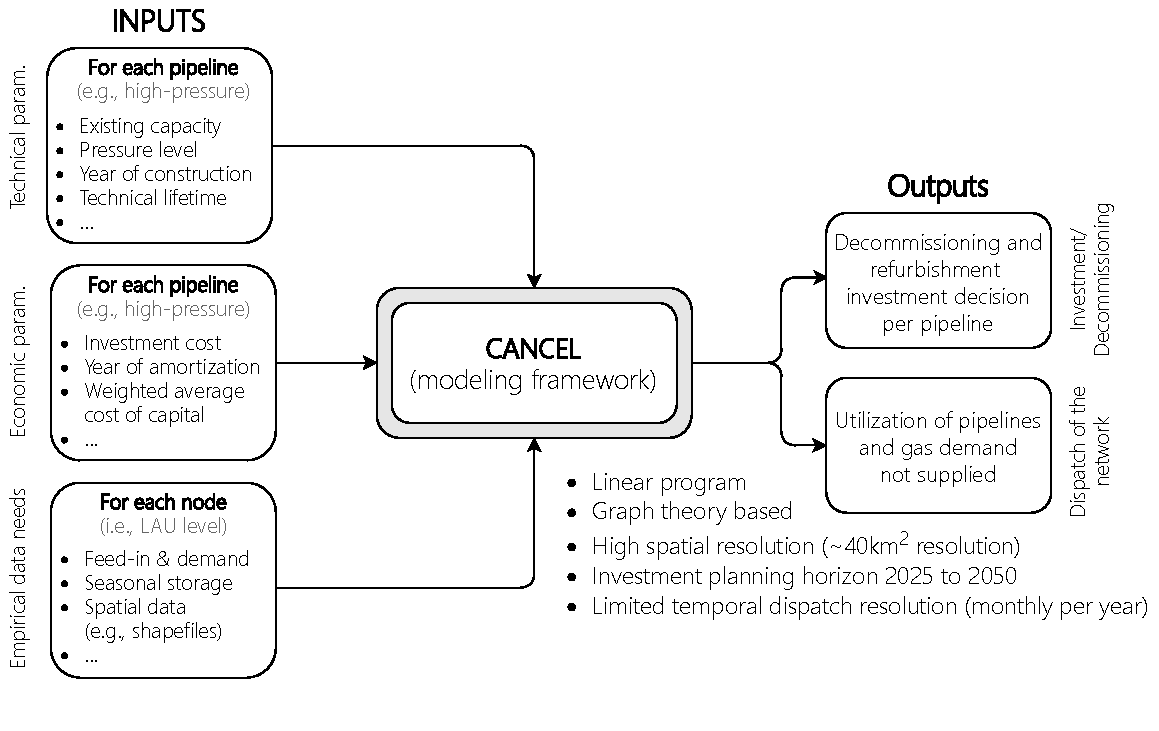
\includegraphics[width=1\linewidth]{flowchart.pdf}
	\caption{Overview of the methodology and developed optimization model \textit{CANCEL} (Cost-effective gAs Network deCommissioning and refurbishment investment dEcision modeL).}
	\label{fig:methodology}
\end{figure}

In the following, selected equations are presented in order to provide an overview of the optimization model. Equation \ref{objective} shows the objective function of the model where $Capex$ is the net present value of the capital expenditures, $Opex$ of the operational expenditures and $Rev$ of the revenues from the supply of gas demand. 
\begin{align}\label{objective}
	\underset{x}{\mathrm{min~}} Capex + Opex - Rev
\end{align}
Besides, $x$ contains the decision variables of the model. Equation \ref{discount} shows the calculation of the discount factor per year $y$ ($\alpha_y$) where $i$ is the interest rate and $y_0$ the reference year. 
\begin{align}\label{discount}
	\alpha_y = \frac{1}{(1+i)^{y-y_0}}
\end{align}
Building upon, $Capex$ is calculated as shown in Equation \ref{eq:capex} where $\omega$ is the weighted average cost of capital (WACC) and $\Pi_y$ the book value of the pipelines in $y$.
\begin{align}\label{eq:capex}
	Capex = \sum_{y} \alpha_y \cdot wacc \cdot \Pi_y
\end{align}
Similar, $Opex$ is calculated as shown in Equation \ref{eq:opex} where $\lambda_y$ are the fixed costs of the pipelines in $y$. 
\begin{align}\label{eq:opex}
	Opex = \sum_{y} \alpha_y \cdot \lambda_y
\end{align}
Equation \ref{eq:lambda} shows the calculation of the $\lambda_y$ where $c^{fix}_{l}$ are the specific fixed costs per $l$ and $\gamma_{l, y}$ the installed pipeline capacity per $l$ in $y$.
\begin{align}\label{eq:lambda}
	\lambda_y = \sum_{l} c^{fix}_{l} \cdot \gamma_{l, y}
\end{align}

In terms of materials and data, we build upon the existing open-source tool \textit{esy-osmfilter} \cite{pluta2020esy} which provides relevant data of the existing European gas network on a high spatial granularity. Furthermore, the open-data platform \textit{energiemosaik} (\url{https://www.energiemosaik.at/intro}) provides helpful information in terms of gas demands at the local level in Austria. Figure \ref{fig:network_west} shows the existing gas network (left) and its representation in the model (right) of the Austrian federal province Vorarlberg. Therein, the two different gas pressure levels high- and mid-pressure are marked in red and green.

\begin{figure}[h]
	\centering
	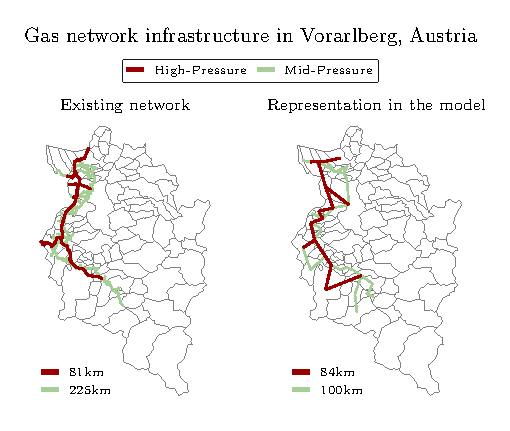
\includegraphics[width=0.95\linewidth]{Network_T8.eps}
	\caption{Existing gas network and its representation in the model of the Austrian federal province Vorarlberg.}
	\label{fig:network_west}
\end{figure}

\section{Preliminary results}
We illustrate the functionality and present preliminary results of the model using a simplified network (see in Figure \ref{fig:a}). The network consists of three nodes (A, B, and C) and two lines (L1 and L2). The planning horizon is between 2020 and 2030, whereby both lines require a refurbishment investment in 2025 in order to provide the gas demand. Node A is the source node in this network. Figure \ref{fig:b} shows the nodal gas supply for varying gas demand and wacc parameter assumptions. Most importantly, it can be seen that the decision to invest in refurbishment depends on both parameters. In particular, a high demand and low wacc as well as low demand and low wacc result in a refurbishment investment decision for both lines L1 and L2 (see top left and right subfigure). In contrast, a high wacc assumption (10\%) leads to no investment decision for refurbishment at line L2 independently from the demand development. Hence, the existing high (and low) gas demand at Node C is not covered (see bottom left and right subfigure) and L2 is decommissioned. The results indicate that both the future gas demand and wacc are key determining parameters in the context of refurbishment investment and decommissioning decisions. At the conference, we will present much more comprehensive results regarding a larger supply area in Austria (as presented in Figure \ref{fig:network_west}). Based on this, we will show which connection lines remain in operation or are decommissioned in the next years.   

\begin{figure}[h]
	\begin{subfigure}[c]{0.3975\textwidth}
		\centering
		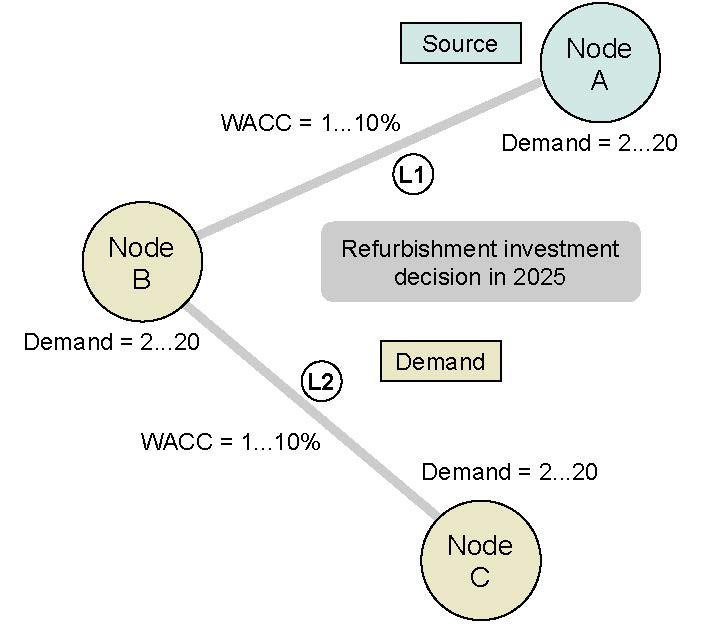
\includegraphics[width=1\linewidth]{FigA.jpg}
		\subcaption{Gas network}
		\label{fig:a}
	\end{subfigure}
	\begin{subfigure}[c]{0.49\textwidth}
		\centering
		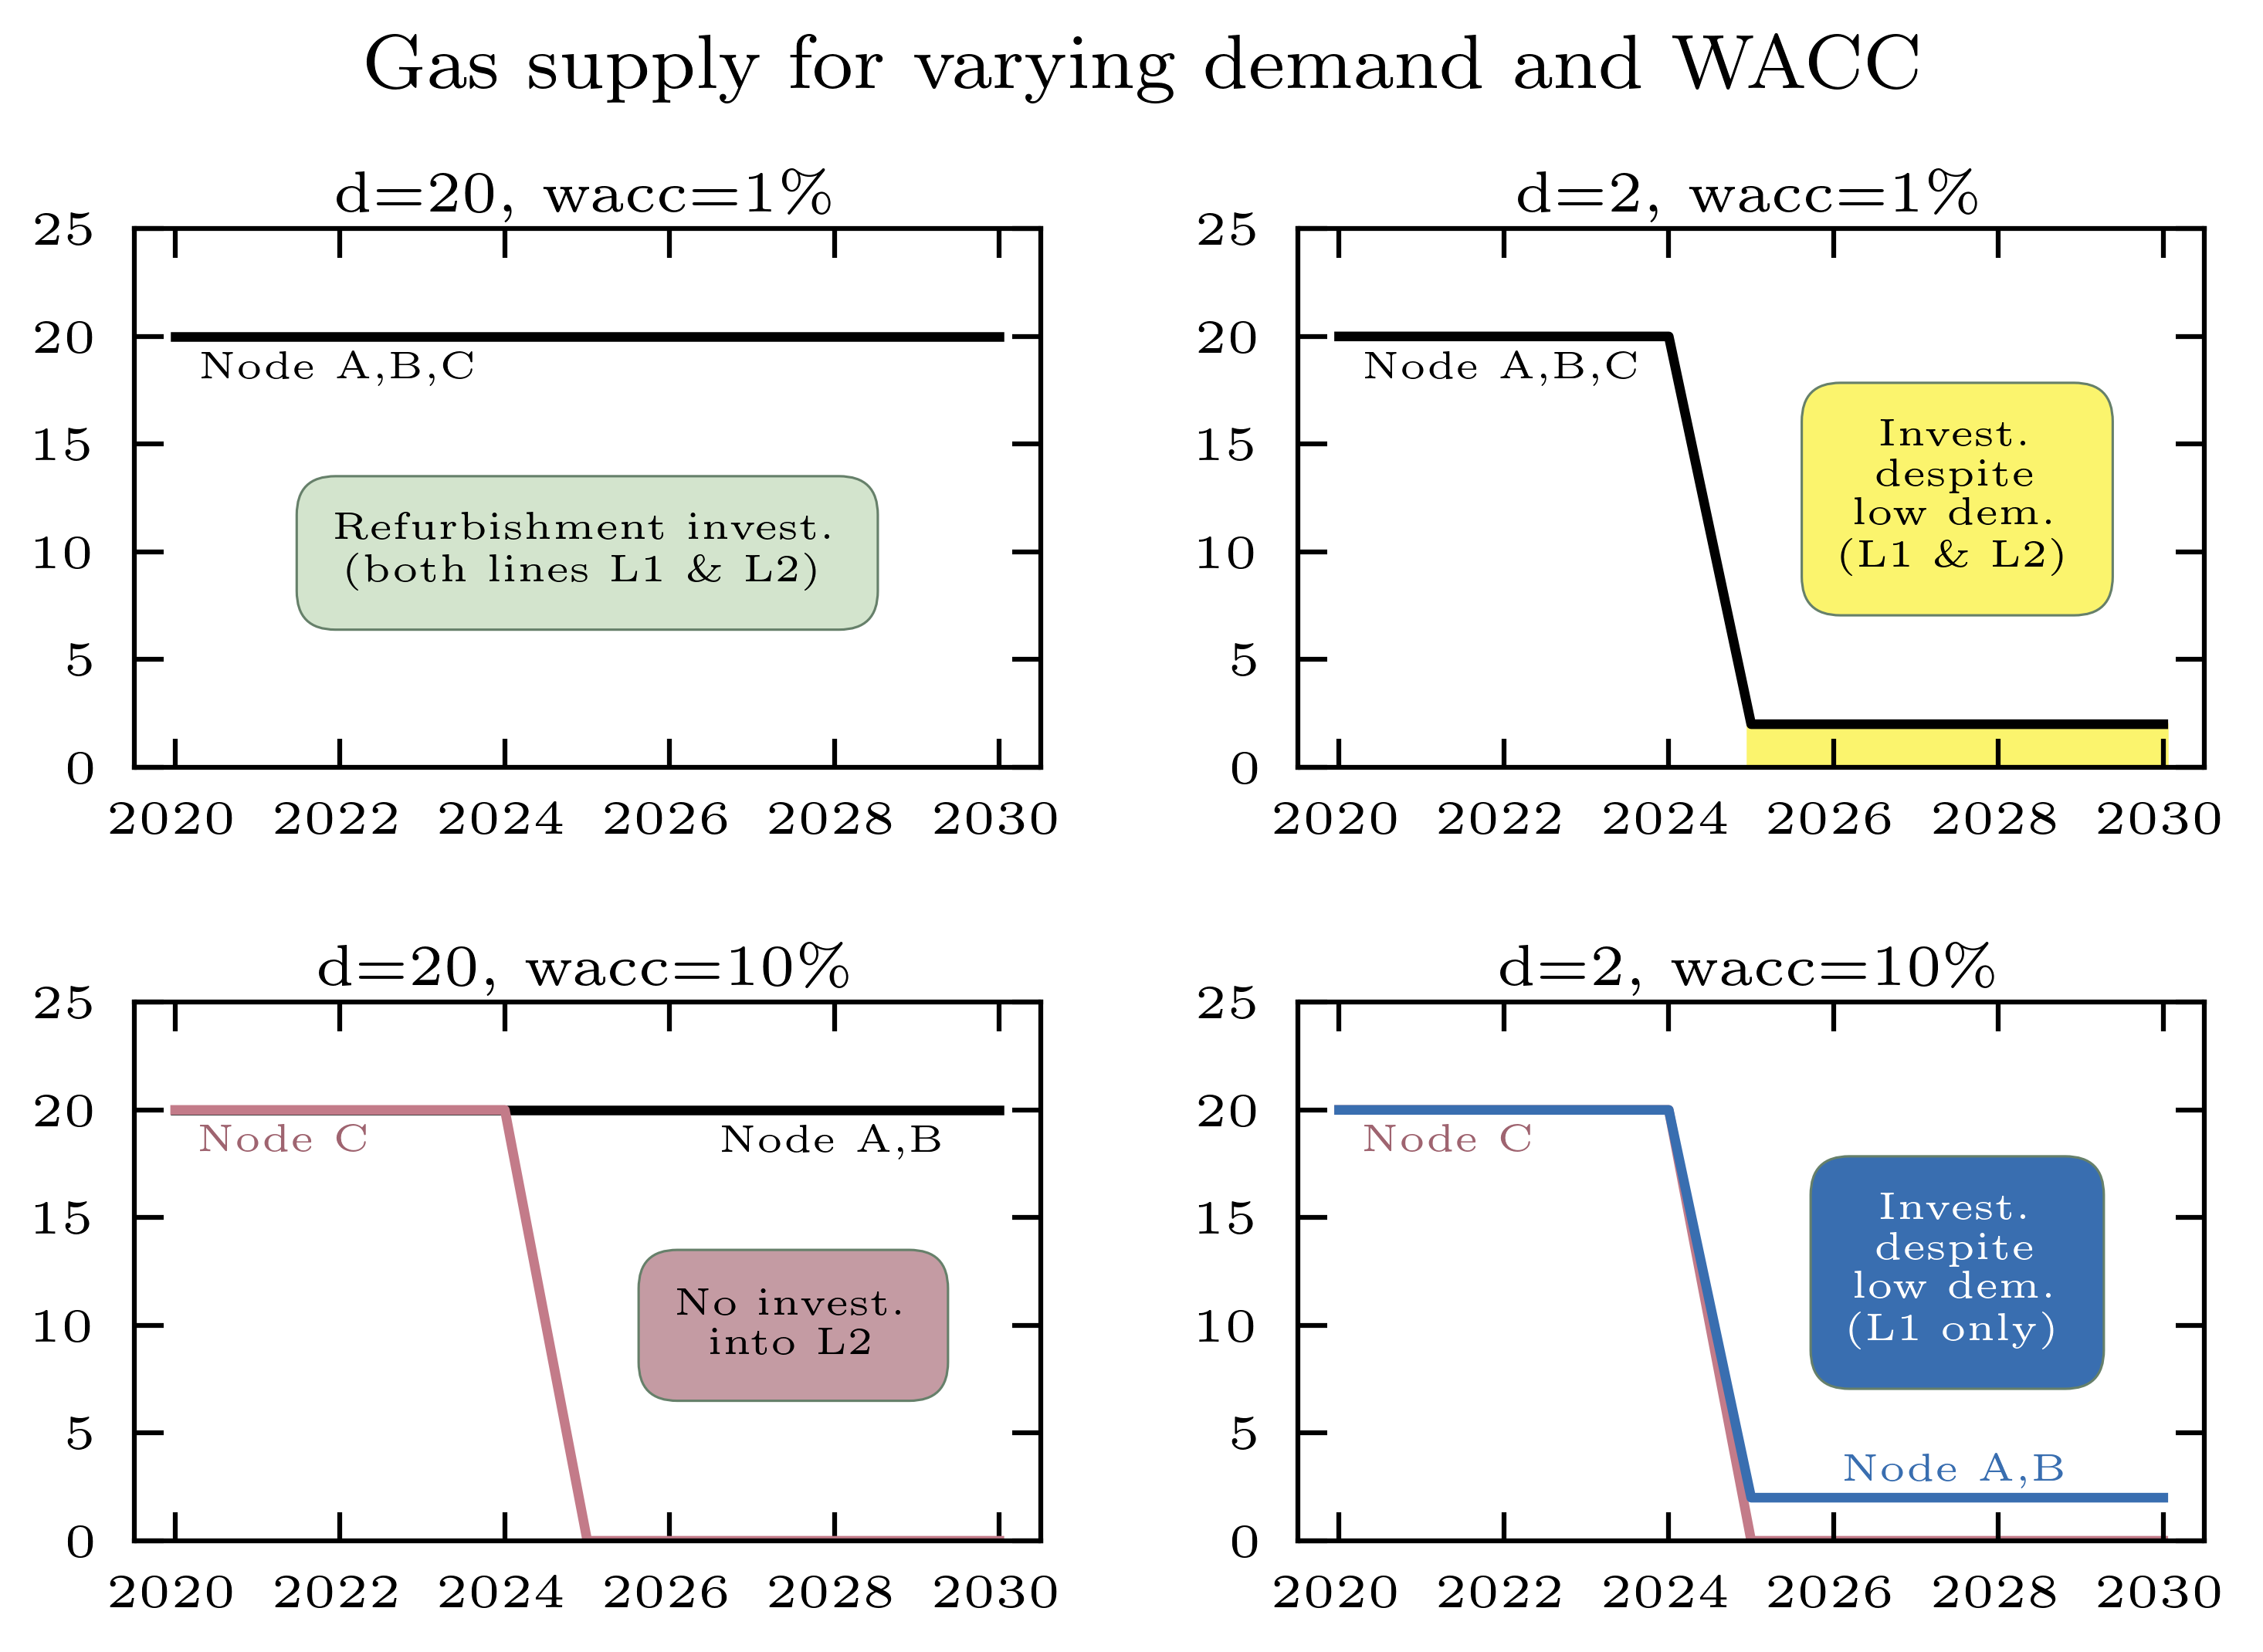
\includegraphics[width=1\linewidth]{FigB.png}
		\subcaption{Varying demand and WACC}
		\label{fig:tenant}
	\end{subfigure}
	\caption{Simplified gas network graph (left) and preliminary results for varying gas demand and weighted average cost of capital (WACC) (right)}
	\label{fig:b}
\end{figure}

{\footnotesize
	\bibliography{mybibfile}
}
\end{document}